\documentclass{article}
\usepackage{amsmath}
\usepackage{tikz}
\usepackage{pgfplots}
\usetikzlibrary{positioning}

\begin{document}

Para un terreno de $x_n$ columnas. 
Donde $i$ es el indice de cada vértice, se pueden calcular sus coordenadas $(x, y)$ 
de manera que cubran una malla rectangular de cualquier dimensión sin desperdiciar  
ningún vértice, con la estrategia de triangle strip. 
Para ello generamos múltiples filas de dos triángulos de alto. 

\begin{center}
	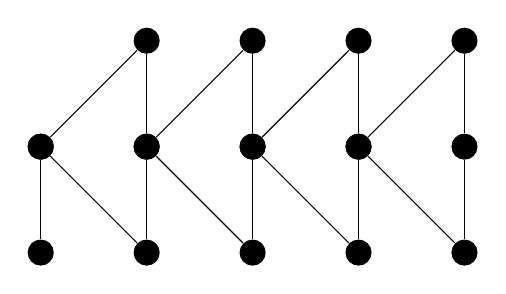
\begin{tikzpicture}[ v/.style= {circle, fill=black }] 
		\node[v] (0) {}; 
		\node[v] (1) [above=of 0]{}; 
		\node[v] (2) [right=of 0]{}; 
		\node[v] (3) [above=of 2]{}; 
		\node[v] (4) [right=of 2]{}; 
		\node[v] (5) [above=of 4]{}; 
		\node[v] (6) [right=of 4]{}; 
		\node[v] (7) [above=of 6]{}; 
		\node[v] (8) [right=of 6]{}; 
		\node[v] (9) [above=of 8]{}; 
		\node[v] (10) [above=of 9]{}; 
		\node[v] (11) [left=of 9]{}; 
		\node[v] (12) [above=of 11]{}; 
		\node[v] (13) [left=of 11]{}; 
		\node[v] (14) [above=of 13]{}; 
		\node[v] (15) [left=of 13]{}; 
		\node[v] (16) [above=of 15]{}; 
		\node[v] (17) [left=of 15]{}; 

		\draw[-] (0) -- (1);
		\draw[-] (1) -- (2);
		\draw[-] (2) -- (3);
		\draw[-] (3) -- (4);
		\draw[-] (4) -- (5);
		\draw[-] (5) -- (6);
		\draw[-] (6) -- (7);
		\draw[-] (7) -- (8);
		\draw[-] (8) -- (9);
		\draw[-] (9) -- (10);
		\draw[-] (10) -- (11);
		\draw[-] (11) -- (12);
		\draw[-] (12) -- (13);
		\draw[-] (13) -- (14);
		\draw[-] (14) -- (15);
		\draw[-] (15) -- (16);
		\draw[-] (16) -- (17);
\end{tikzpicture}
\end{center}

De esta manera si  se apilan las filas con un corrimiento de 2 puntos hacia arriba
se puede generar una malla que cubra la superficie completamente. Me refiero a esta figura como fila doble a partir de ahora.

Para obtener los indices podemos usar las siguientes formulas.

\begin{equation*}
	n = 4x_n-2
\end{equation*}
Cantidad de vértices en la fila doble.

\begin{equation*}
	r = i \% n
\end{equation*}
Indice del vértice local a la fila doble.

\begin{equation*}
	c = \Bigl\lfloor \frac{r}{2} \Bigr\rfloor
\end{equation*}
Columna a la que pertenecería el vértice en una fila simple.

\begin{equation*}
	d = \Bigl\lfloor \frac{c}{x_n} \Bigr\rfloor\%2
\end{equation*}
Dirección en la que está creciendo la fila. 0 si va  a la derecha, 1 si vuelve.

\begin{equation*}
	s = 1-2d
\end{equation*}
La dirección expresada como signo 1 si va, -1 si vuelve.

\vspace{0.5cm}

Para generar la coordenada $y$ combino 3 cálculos.

\begin{equation*}
    s(i\%2)
\end{equation*}
Genera la oscilación entre puntos consecutivos. Cuando la fila va los vértices pares 
quedan abajo y los impares arriba. Cuando vuelve es lo contrario.

\begin{equation*}
    \Bigl\lfloor \frac{c}{x_n} \Bigr\rfloor 2
\end{equation*}
Genera el corrimiento hacia arriba dentro de la fila doble para que vuelva un punto mas
arriba de lo que fue.

\begin{equation*}
	\Bigl\lfloor \frac{i}{n} \Bigr\rfloor 2
\end{equation*}
Genera un corrimiento de 2 puntos entre filas dobles para cubrir el terreno y no 
superponerse.

\begin{equation*}
    y = s(i\%2) +
	 \Bigl\lfloor \frac{c}{x_n} \Bigr\rfloor 2 +
	 \Bigl\lfloor \frac{i}{n} \Bigr\rfloor 2
\end{equation*}
Sumando estos cálculos obtenemos la coordenada $y$.

\vspace{0.5cm}

La forma típica de convertir los indices en columnas es mediante el modulo. 

\begin{equation*}
    x =  \Bigl\lfloor \frac{r}{2} \Bigr\rfloor
\end{equation*}
Obteniendo este comportamiento.
\begin{figure}[h]
    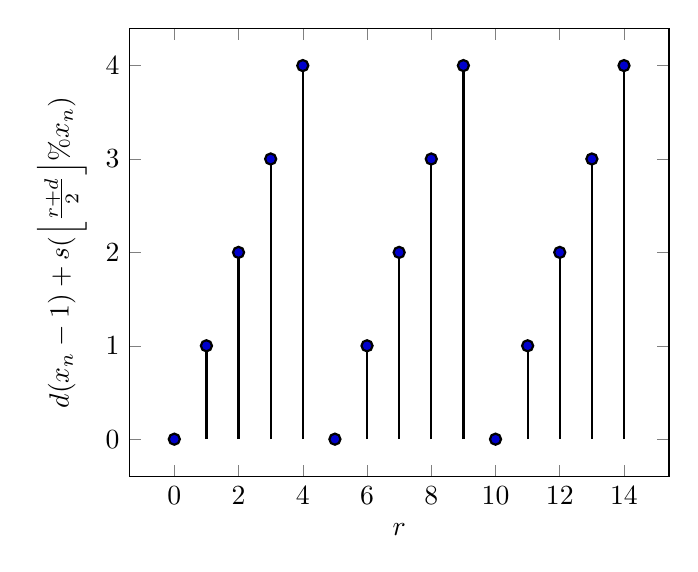
\begin{tikzpicture}
        \begin{axis}[
            domain = 0:14,
            samples = 15,
            xlabel={$r$},
            ylabel={$d(x_n-1)+s ( \Bigl\lfloor \frac{r+d}{2} \Bigr\rfloor \% x_n )$}]
				\addplot+[ycomb,black,thick] {mod(x, 5)};
        \end{axis}
    \end{tikzpicture}
\end{figure}
Esto sirve para filas simples que solo van, pero queremos filas que van y vuelven.

\vspace{0.5cm}

Si usamos el signo que calculamos antes podemos invertir el gráfico para cuando la fila 
vuelve, calculando así la coordenada x.
\begin{equation*}
    x = d(x_n-1)+s ( \Bigl\lfloor \frac{r+d}{2} \Bigr\rfloor \% x_n )
\end{equation*}
Obteniendo este comportamiento.

\begin{figure}[h]
    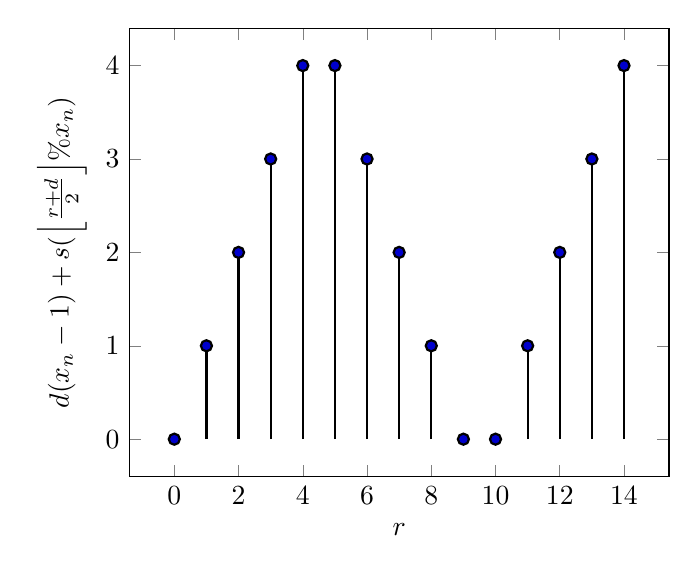
\begin{tikzpicture}
        \begin{axis}[
            domain = 0:14,
            samples = 15,
            xlabel={$r$},
            ylabel={$d(x_n-1)+s ( \Bigl\lfloor \frac{r+d}{2} \Bigr\rfloor \% x_n )$}]
				\addplot+[ycomb,black,thick] { 
				mod(floor(x/5),2)*4
				+ (1-2*mod(floor(x/5),2)) * mod(x, 5)};
        \end{axis}
    \end{tikzpicture}
\end{figure}

\newpage

En conclusión podemos calcular las coordenadas $(x, y)$ con las formulas.

\begin{equation*}
    y = s(i\%2) +
	 \Bigl\lfloor \frac{c}{x_n} \Bigr\rfloor 2 +
	 \Bigl\lfloor \frac{i}{n} \Bigr\rfloor 2
\end{equation*}

\begin{equation*}
    x = d(x_n-1)+s ( \Bigl\lfloor \frac{r+d}{2} \Bigr\rfloor \% x_n )
\end{equation*}

En el código formulas.py hay un ejemplo de implementación.

\end{document}
